\documentclass{article}
\usepackage{amsmath}
\usepackage{mathtools}

\begin{document}
\section{Introduction}
\textbf{Accurate and stable stochastic estimation of the parameter gradient of the energy expectation value, $\partial E/\partial p$, is an integral component of variational Monte Carlo (VMC) wave function energy optimization techniques \cite{PhysRevB.64.024512, doi:10.1063/1.1604379, Toulouse2007}.}
Within these techniques, wave function parameters are updated iteratively, with the estimate of $\partial E/\partial p$ used in determining updates.
If the estimation is inaccurate, having a large bias, the final converged wave function is not guaranteed to be the lowest energy wave function in the parameterization space.
If the estimation is unstable, having a large variance, the updates will have large statistical fluctuations, decreasing efficiency.
An appropriate estimator for $\partial E/ \partial p$ should then have both low bias and variance, leading to efficient optimization and a final wave function with minimum energy in the parameterization space.

A useful starting point is the naive Monte Carlo estimator for $\partial E/\partial p$ evaluated on a wave function $\Psi(p, R)$ 
\begin{equation}
\hat{\theta}^M \equiv \frac{2}{M}\sum_{i=1}^M \frac{\hat{H}\Psi}{\Psi}(R_i) \frac{\partial_p \Psi}{\Psi}(R_i) - \frac{2}{M-1} \sum_{i=1}^M \Big(\frac{1}{M} \sum_{j=1}^M \frac{\hat{H}\Psi}{\Psi}(R_j)\Big)\frac{\partial_p \Psi}{\Psi}(R_i). \label{eq:naive_estimator}
\end{equation}
The sums are over $M$ configurations drawn from the distribution $|\Psi(p, R)|^2$, and $\hat{H}$ is the Hamiltonian operator.
\textbf{While unbiased, $\hat{\theta}^M$ has a well documented divergent variance \cite{Avella} due to the behavior of the first term in \eqref{eq:naive_estimator} near the nodes of $\Psi$.}
This infinite variance leads to inefficient optimization and has prompted a search for zero bias, finite variance estimators of $\partial E/\partial p$.

\textbf{Current zero bias, finite variance estimation techniques involve guiding or auxiliary wave functions, such as a reweighting scheme \cite{Avella, Attaccalite2008} or the improved estimators of Assaraf and Caffarel \cite{doi:10.1063/1.1286598, Assaraf2003}.}
While zero bias is achieved for arbitrary guiding wave functions $\Psi_G$, finite variance is only acquired with specially tuned guiding functions which cancel the divergences in \eqref{eq:naive_estimator} near the nodes of $\Psi$.
A general form for $\Psi_G$ which yields a finite-variance estimate of $\partial E/\partial p$ is provided by Umrigar \cite{doi:10.1063/1.4933112} where $\Psi_G$ differs from $\Psi$ only near the nodes, the prior having a finite value.
Still unresolved is a zero bias, finite variance estimator for \eqref{eq:naive_estimator} without the luggage of a guiding wave function. 

\textbf{We derive and test a simple regularized estimator for $\partial E/\partial p$ which has finite variance, can be extrapolated to zero bias, and does not rely on guiding wave functions.}
Instead, the divergence in the first term of \eqref{eq:naive_estimator} is suppressed via multiplication by a polynomial function within a distance $\epsilon$ of the nodes of $\Psi(p, R)$. 
We present rigorous mathematical proofs for the scalings of the variance and bias of the regularized estimator with $\epsilon$, and provide an algorithm for the zero bias extrapolation of the estimate.
The mathematical predictions and extrapolation procedure are then tested in evaluating $\partial E/\partial p$ for a multi-Slater-Jastrow (MSJ) trial wave function on the LiH molecule.

\section{Regularized estimator}
As mentioned before, the naive estimator \eqref{eq:naive_estimator} suffers from an infinite variance. 
\textbf{The divergent contribution to the variance arises from the evaluation of the integral
\begin{equation}
\int \Big(\frac{\hat{H}\Psi}{\Psi}\frac{\partial_p\Psi}{\Psi}\Big)^2 |\Psi|^2 dR.
\label{eq:divergent_integral}
\end{equation}
when $\Psi$ is not an eigenstate of $\hat{H}$ and the parameter $p$ affects the nodes of $\Psi$, such as orbital or determinantal coefficients.}
In this case, to lowest order in distance $|R-N|$ near a nodal point $N$ of $\Psi$, both $\hat{H}\Psi$ and $\partial_p \Psi \sim const$ and $\Psi \sim \nabla \Psi(N) \cdot (R - N)$, leading to the integrand in \eqref{eq:divergent_integral} behaving as $1/|R-N|^2$ near the nodes of $\Psi$.
Since the integration domain includes the nodal surface of $\Psi$, the $1/|R-N|^2$ behavior of the integrand as $|R-N|\rightarrow 0$ leads to a divergent integral.

\textbf{Multiplying the first term in the naive estimator \eqref{eq:naive_estimator} by a function $f_\epsilon$ yields a finite variance estimator of $\partial E/\partial p$}
\begin{equation}
\hat{\theta_\epsilon}^M \equiv \frac{2}{M}\sum_{i=1}^M \frac{\hat{H}\Psi}{\Psi}(R_i)\frac{\partial_p \Psi}{\Psi}(R_i) f_\epsilon(R_i) - \frac{2}{M-1} \sum_{i=1}^M \Big(\frac{1}{M} \sum_{j=1}^M \frac{\hat{H}\Psi}{\Psi}(R_j)\Big)\frac{\partial_p \Psi}{\Psi}(R_i), \label{eq:regularized_estimator}
\end{equation}
where 
\begin{equation}
f_\epsilon(R) = \begin{cases} 
      O(|\frac{x}{\epsilon}|) & |\frac{x}{\epsilon}| < 1 \\
      1 & |\frac{x}{\epsilon}| \ge 1 \\
   \end{cases},\ x \equiv \frac{\nabla \Psi(R) \Psi(R)}{|\nabla \Psi(R)|^2}.
\label{eq:regularizing_function}
\end{equation} 
The previously divergent contribution to the estimator variance \eqref{eq:divergent_integral} is replaced by a finite integral, verified by piecewise integration
\begin{equation}
\int \Big(\frac{\hat{H}\Psi}{\Psi}\frac{\partial_p\Psi}{\Psi}\Big)^2 f_\epsilon^2 |\Psi|^2 dR =\int_{|x/\epsilon|\geq 1} \Big(\frac{\hat{H}\Psi}{\Psi}\frac{\partial_p\Psi}{\Psi}\Big)^2 |\Psi|^2 dR + \int_{|x/\epsilon|< 1} \Big(\frac{\hat{H}\Psi}{\Psi}\frac{\partial_p\Psi}{\Psi}\Big)^2 f_\epsilon^2 |\Psi|^2 dR,
\label{eq:convergent_integral}
\end{equation}
Since $\Psi = 0$ only occurs when $x = 0$, the integral for $|x/\epsilon|\geq 1$ completely excludes the nodal surface of $\Psi$, and is finite. 
Further, since $|x/\epsilon| \sim |\nabla\Psi(N) \cdot (R-N)|/\epsilon|\nabla  \Psi(N)|$ as $|R - N| \rightarrow 0$, the integrand arbitrarily close to the nodal surface is a constant, meaning the second integral for $|x/\epsilon| < 1$ is also finite.

\textbf{A more careful analysis shows the variance of \eqref{eq:regularized_estimator} is not only finite, but decreases exponentially as $1/\epsilon$ to lowest order in $\epsilon$ for any choice of $f_\epsilon$ satisfying the conditions in \eqref{eq:regularizing_function}.}
This is a consequence of the non-dimensionality of $f_\epsilon$ which ensures that all contributions to the $|x/\epsilon|< 1$ integral in \eqref{eq:convergent_integral} take the form:
\begin{equation}
\int_{|x/\epsilon|< 1} \Big(\frac{\hat{H}\Psi}{\Psi}\frac{\partial_p\Psi}{\Psi}\Big)^2 |\frac{x}{\epsilon}|^n |\Psi|^2 dR, n\geq 2
\end{equation}
As $\epsilon \rightarrow 0$, the integration domain is very near the nodal surface and the integrand can be Taylor expanded to lowest order in $|R-N|$. 
The Taylor expansion yields an integrand $|x/\epsilon|^{n-2}/\epsilon^2$ and results in an integral which scales as $O(1/\epsilon)$ to lowest order in $\epsilon$.

\textbf{Continuing this analysis, we find that the regularized estimator results in a linear-order biased estimation of $\partial E/\partial p$ for a general function $f_\epsilon$ satisfying \eqref{eq:regularizing_function}.}
The bias in \eqref{eq:regularized_estimator} results only from the first term and is written as 
\begin{equation}
\text{Bias: } \int_{|x/\epsilon|< 1} \Big(\frac{\hat{H}\Psi}{\Psi}\frac{\partial_p\Psi}{\Psi}\Big) (f_\epsilon - 1)|\Psi|^2 dR.
\label{eq:estimator_bias}
\end{equation}
As before, we take $\epsilon \rightarrow 0$ and Taylor expand the integrand to lowest order in $|R-N|$.
This yields an integrand, to lowest order in $\epsilon$, $c|x/\epsilon| - 1$ where $c$ is an arbitrary constant.
Carrying out the integration yields a bias that scales as $O(\epsilon)$ to lowest order in $\epsilon$.
The linear bias is inhibitive to zero bias extrapolation as the estimation bias is present for any value of $\epsilon$ while the variance increases exponentially with $\epsilon \rightarrow 0$.

\textbf{A simple normalization condition on $f_\epsilon$ ensures a bias of $O(\epsilon^3)$, allowing for efficient extrapolation to zero bias.}
The expression for the bias \eqref{eq:estimator_bias} as $\epsilon \rightarrow 0$ after carrying out the necessary Taylor expansions is
$$
\lim_{\epsilon\rightarrow 0}\text{Bias} =  A \int_{|x/\epsilon|< 1} (f_\epsilon - 1) dR.
$$
where $A$ is a constant resulting from $\hat{H}\Psi$ and $\partial_p \Psi \sim const$ as $|R-N|\rightarrow 0$.
As such, the linear order bias can be removed by enforcing a normalization condition on $f_\epsilon$ on the domain of integration, 
\begin{equation}
\int_{|x/\epsilon|< 1} (f_\epsilon - 1) dR = 0.
\label{eq:normalization_condition}
\end{equation}
The leading order contribution to the bias arises from the breakdown of the Taylor approximation $\hat{H}\Psi$ and $\partial_p \Psi \sim const$, and results in a bias $O(\epsilon^3)$.
The quadratic contribution to the bias is zero as $f_\epsilon$ is even in $(R-N)$.

\textbf{The last set of continuity and smoothness conditions on $f_\epsilon$ at $|x/\epsilon| = 1$ reduce the magnitude of the cubic bias.}
These two conditions can be written as 
\begin{equation}
f(1) = 1, \nabla f(1) = 0.
\label{eq:smoothness_condition}
\end{equation}
The three conditions, smoothness, continuity and normalization, can all be satisfied with a polynomial formula for $f$
\begin{equation}
f_\epsilon(|\frac{x}{\epsilon}|) = 7(\frac{x}{\epsilon})^6 - 15(\frac{x}{\epsilon})^4 + 9(\frac{x}{\epsilon})^2.
\label{eq:final_regularization}
\end{equation}
Therefore, the regularized estimator \eqref{eq:regularized_estimator} with $f_\epsilon$ defined as \eqref{eq:final_regularization} serves as a finite variance estimator for $\partial E/\partial p$ which has a leading order cubic bias in $\epsilon$.

\textbf{With the regularized estimator in hand, the finite variance, zero bias, extrapolated estimation for $\partial E/\partial p$ using can be carried out in four steps.}
First, conduct a standard VMC calculation with probability distribution $|\Psi|^2$ to the generate configurations $\{R_i\}$ needed for estimation.
Second, evaluate the distance $x_i$ as defined in \eqref{eq:regularizing_function} for each configuration $R_i$.
Third, calculate the regularized estimate \eqref{eq:regularized_estimator} on the set of configurations for a sequence of increasing $\epsilon$.
Fourth, fit a function $a\epsilon^3 + b$ to the estimated values; the intercept $b$ is then a zero bias estimate for $\partial E/\partial p.$

\section{Application to LiH molecule}
\textbf{We test the effectiveness of the regularized estimator in evaluating $\partial E/\partial p$ for the determinantal coefficients of a multi-Slater Jastrow (MSJ) wave function for the LiH molecule.}
A full configuration interaction expansion over Li 1s, 2s, 2p and H 1s orbitals was chosen for the multi-Slater expansion.
The orbitals were constructed from a restricted open-shell Hartree Fock calculation using a correlation consistent quadruple-zeta valence basis set \textbf{ref}.
An unoptimized 2-body Jastrow function with electron-electron cusp conditions of the form in \textbf{ref} was used.
The wave function is meant to be a typical starting point for VMC optimization of the Jastrow and determinantal coefficients, and a useful playground to test the regularized estimator when evaluating $\partial E/\partial p$ for determinantal coefficients.

\textbf{Figure 1 illustrates how the regularized estimator removes the divergence present in the integral \eqref{eq:divergent_integral} across a node of $\Psi$ when $p$ is a determinantal coefficient }
In the lower plot the logarithm of the regularized integrand \eqref{eq:convergent_integral} is shown for various $\epsilon$ along a path normal to a node of the wave function $\Psi$.
The normal coordinate to the node is $x$.
For all values of $\epsilon$, the value of the integrand is pushed to zero at the node, removing the divergence in the integral.
The sharp increase in the integrand near $x=0$ as $\epsilon$ decreases is indicative of the exponential increase in the value of this integrand as $\epsilon \rightarrow 0$.
Shown in the upper figure is the first term in \eqref{eq:regularized_estimator} across the node, exhibiting no divergences.

\textbf{By integrating across the normal coordinate $x$, the predicted $O(1/\epsilon)$, $O(\epsilon^3)$ scalings of the variance and bias are recovered, as shown in Figure 2.} 
The integration for both the bias and variance are carried out for the path shown in Figure 1 from $x = -0.1$ to $0.1$ Bohr and normalized by a factor $\int |\Psi|^2 dR$ along that path.
The blue dots correspond to the values of the integrals for different values of $\epsilon$ and the orange dashed lines are fits to the predicted scaling functions with respect to $\epsilon$.
The predicted cubic bias is observed for six decades in $\epsilon$ while the exponential decrease in variance stands for four decades.
The increase in the variance after $\epsilon = 10^{-2}$ occurs due to the breakdown of the assumption $\Psi(R) \sim \nabla(N) \cdot (R-N)$, resulting in a linear increase in variance with $\epsilon$.
This change is not mirrored in the bias since the sub-leading order scaling with $\epsilon$ appears in the bias when the assumptions of $\hat{H}\Psi$ and $\partial_p \Psi \sim const$ break down.

\textbf{In Figure 3 we demonstrate the zero bias, finite-variance extrapolation for $\partial E/\partial p$ using the regularized estimator.}
The four step procedure outlined in the previous section was carried out.
A standard VMC calculation with 200,000 steps and 2,000 configurations per step were first collected.
Then $\partial E/\partial p$ was estimated using \eqref{eq:regularized_estimator} for $\epsilon$ between $10^{-1}$ Bohr and $10^{-5}$ Bohr, shown in the blue data points.
Since the same configurations were used for each evaluation, the blue data points have a strong statistical correlation and the predicted $\epsilon^3$ bias is very clearly present, shown by the orange fit curve.
The intercept of the fit curve is shown by the red star and is the zero-bias estimate of $\partial E/\partial p$; the variance can be deduced by the error bar of the blue data points, in this case 0.025 mHa.
Note that the extrapolation is not strictly necessary as the bias is zero within statistical errors for small values of $\epsilon$, meaning that most practical calculations can be carried out for a fixed value of $\epsilon$ between $10^{-5}$ and $10^{-2}$ Bohr.

\section{Conclusion}
\textbf{Integral to the reliability of variational Monte Carlo wave function optimization methods is the finite variance estimation of $\partial E/\partial p$.}
Within these techniques, wave function parameters are updated iteratively, with the estimate of $\partial E/\partial p$ used in determining updates.
If the estimation is inaccurate, having a large bias, the final converged wave function is not guaranteed to be the lowest energy wave function in the parameterization space.
If the estimation is unstable, having a large variance, the updates will have large statistical fluctuations, decreasing efficiency.
While the naive Monte Carlo estimator for $\partial E/\partial p$ is unbiased, it has an infinite variance, prompting a search for finite variance estimators for the quantity.

\textbf{In this work, we derive and test a simple regularized estimator for $\partial E/\partial p$ which has finite variance and can be extrapolated to zero bias.}
The divergent variance present in the naive Monte Carlo estimator is suppressed via multiplication by a polynomial function within a distance $\epsilon$ of the nodes of $\Psi(p, R)$. 
We prove that the regularized estimator manages a finite variance by incurring a cubic bias which can be efficiently extrapolated to zero bias.
The extrapolation is carried out, and a finite variance, zero-bias estimate of $\partial E/\partial p$ is evaluated for a determinantal coefficient in a trial wave function for the LiH molecule.


\section{Figures}
\begin{figure*}
\centering
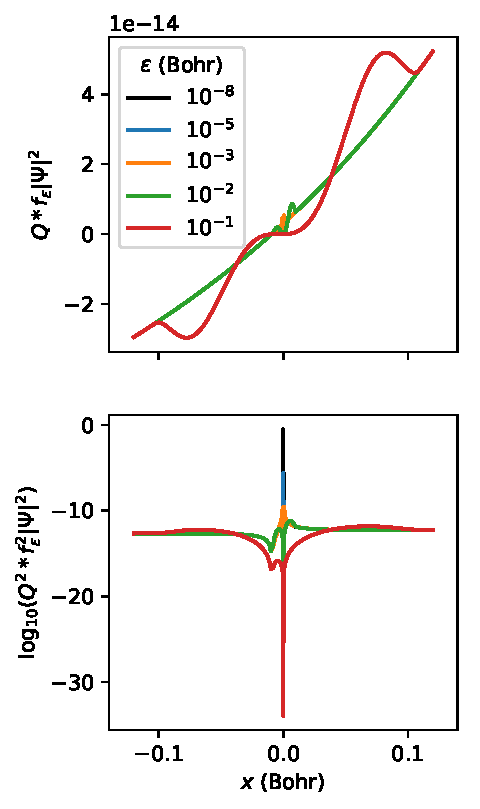
\includegraphics{../2_plots/viznode.pdf}
\caption{$\frac{\hat{H}\Psi}{\Psi}\frac{\partial_p \Psi}{\Psi} f_\epsilon$ and logarithm $(\frac{\hat{H}\Psi}{\Psi}\frac{\partial_p \Psi}{\Psi} f_\epsilon)^2$, plotted against the normal coordinate $x$ from a node of $\Psi$. Curve colors correspond to different values of $\epsilon$ ranging from $10^{-1}$ to $10^{-8}$ Bohr.}
\end{figure*}

\begin{figure*}
\centering
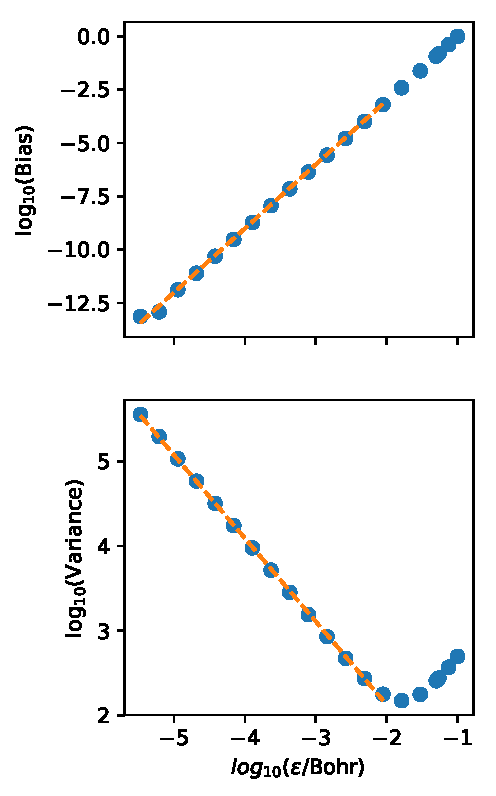
\includegraphics{../2_plots/integratenode.pdf}
\caption{Scaled bias and variance of $\frac{\hat{H}\Psi \partial_p \Psi}{\Psi^2}$ evaluated by numerical integration from $r = -0.1$ to $r = 0.1$ across the node in Figure 1. The blue dots are the numerically integrated values and the orange curves indicate best fits to the functions $a\epsilon^3$ and $b + c/\epsilon$ for the bias and variance, respectively.}
\end{figure*}

\begin{figure*}
\centering
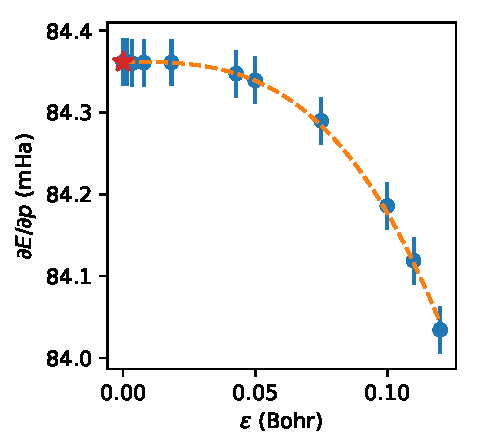
\includegraphics{../2_plots/dedp.pdf}
\caption{Zero bias, finite variance extrapolation for $\partial E/\partial p$ using the regularized estimator. The blue points are evaluated using VMC, the orange curve is a fit to $a + b\epsilon^3$, and the red star denotes the extrapolated estimation. }
\end{figure*}
\pagebreak

\bibliographystyle{unsrt}
\bibliography{pgradregr}
\end{document}